\documentclass[11pt,a4paper]{article}
\usepackage[utf8]{inputenc}
\usepackage[T1]{fontenc}
\usepackage{amsmath}
\usepackage[usenames,dvipsnames,svgnames,table]{xcolor}
\usepackage[normalem]{ulem}
\usepackage[left=1.00cm, right=1.00cm, top=0.40cm, bottom=0.2cm]{geometry}
\PassOptionsToPackage{defaults=hu-min}{magyar.ldf}
\usepackage[magyar]{babel}
\usepackage{framed, fancyhdr, wasysym, graphicx, multirow, hyperref}

\begin{document}
\renewcommand{\labelitemi}{\textbullet}
\def\br{\\[0.1cm]}
\thispagestyle{empty}
\begin{center}
	\colorbox{lightgray}{{\large JPSMA3} \hspace{3cm} {\large Webes alkalmazások fejlesztése 1. beadandó} \hspace{5cm} \thepage}
\end{center}
\begin{framed}
	\begin{flushleft}
		{\large \textbf{Bauer Bence}}
		\hspace{3cm}{\large \textbf{1.Beadandó/9.Feladat}}
		\hspace{5.4cm}{\large 2019.03.13.}\br
		{\large JPSMA3}\br
		{\large \href{mailto:bauerbence5@gmail.com}{bauerbence5@gmail.com}}
	\end{flushleft}
\end{framed}
\section{Feladat}

Készítsünk egy mozi üzemeltető rendszert, amely alkalmas az előadások, illetve
jegyvásárlások kezelésére.
\begin{itemize}
	\item A webes felületen keresztül a nézők tekinthetik meg a moziműsort,
	valamint rendelhetnek jegyeket.
	\item A főoldalon megjelenik a napi program, azaz mely filmeket mikor
	vetítik a moziban, valamint kiemelve az öt legfrissebb (legutoljára
	felvitt) film plakátja.
	\item A filmet kiválasztva megjelenik annak részletes leírása (rendező,
	főszereplők, hossz, szinopszis), plakátja, továbbá az összes előadás
	időpontja.
	\item Az időpontot kiválasztva lehetőség nyílik helyfoglalásra az
	adott előadásra.
	Ekkor a felhasználónak meg kell adnia a lefoglalandó ülések helyzetét (sor,
	illetve oszlop) egy, a mozitermet sematikusan ábrázoló grafikus felületen.
	\item Egyszerre legfeljebb 6 jegy foglalható, és természetesen csak a
	szabad helyek foglalhatóak (amelyek nem foglaltak, vagy eladottak).
	A felhasználónak ezen felül meg kell adnia teljes nevét, valamint
	telefonszámát, ezzel véglegesíti a foglalást.
\end{itemize}
Az adatbázis az alábbi adatokat tárolja:
\begin{itemize}
	\item filmek (cím, rendező, szinopszis, hossz, plakát, bevitel dátuma)
	\item termek (név, sorok száma, oszlopok száma)
	\item előadások (film, kezdő időpont, terem)
	\item helyek (előadás, terem, sor, oszlop, státusz
	<szabad, foglalt, eladott>, foglaló, neve, foglaló telefonszáma)
	\item alkalmazottak (teljes név, felhasználónév, jelszó)
\end{itemize}
\section{Elemzés}
\begin{itemize}
	\item Az alkalmazás perzisztencia részét egy külső C\# könyvtárként
	kezeljük. A weblap részt MVC segítségével hozzuk létre.
	\item Több oldalra (Nézetek) is szükségünk van:
	\begin{itemize}
		\item Főoldal a legújabb filmekkel és az aznapi műsorokkal (Home/Index)
		\item Egy összes filmet kilistázó oldal (Movie/Index)
		\item Filmek részletes leírására szolgáló oldal (Movie/Details)
		\item Mozitermet ábrázoló felület, ahol a felhasználó helyet tud
		foglalni az előadásra (Movie/Reserve)
	\end{itemize}
	\item Az alkalmazáshoz szükséges egy adatbázis is. A feladatban leírt
	adatbázis jól megfogalmazható SQL adatbázisként.
\end{itemize}
\newpage
\thispagestyle{empty}
\begin{center}
	\colorbox{lightgray}{{\large JPSMA3} \hspace{3cm} {\large Webes alkalmazások fejlesztése 1. beadandó} \hspace{5cm} \thepage}
\end{center}
\begin{figure}[h]
	\centering
	\includegraphics[width=12cm]{umls/UseCase.png}
	\caption{Felhasználói eset diagram}
\end{figure}
\section{Tervezés}
\begin{itemize}
	\item Programszerkezet: A programot egy Model-View-Controller architektúrát
	alkalmazó alkalmazással valósítjuk meg.
	\item Nézetekhez tartozó kontrollerek:
	\begin{itemize}
		\item Home - Biztosítja a kezdőoldalon a lista feltöltését.
		\item Movie - Filmek listázásához, egy film részletes adataihoz illetve
		helyfoglaláshoz állítja össze az adatokat.
	\end{itemize}
	\begin{figure}[h]
		\centering
		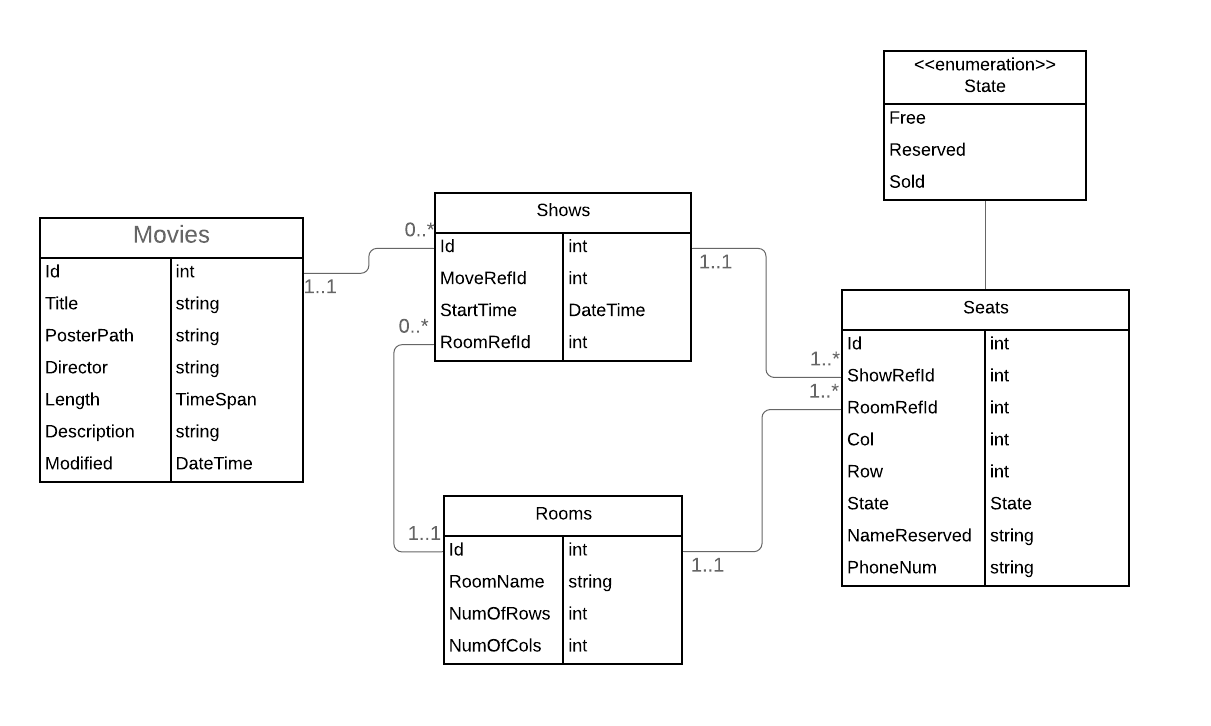
\includegraphics[width=18cm]{umls/Entity.png}
		\caption{Adatbázis felépítése}
	\end{figure}
	\newpage
	\thispagestyle{empty}
	\begin{center}
	\colorbox{lightgray}{{\large JPSMA3} \hspace{3cm} {\large Webes alkalmazások fejlesztése 1. beadandó} \hspace{5cm} \thepage}
	\end{center}
	\begin{figure}[h]
	\centering
	\includegraphics[width=16cm]{umls/Class.png}
	\caption{Osztálydiagram}
	\end{figure}
	\item Nézetmodellek leírása:
	\begin{itemize}
		\item\verb|MovieIndexViewModel|: A főoldalhoz összegyűjti az 5 legújabb
		filmet és az aznapi vetítések adatait.
		\item\verb|MovieDetailsViewModel|: A kiválasztott filmhez összegyűjti a
		film részletes adatait, a film vetítési idejeit illetve a termek neveit.
		\item\verb|Reservation|: A kiválasztott előadásra előkészíti a hozzá
		tartozó ülőhelyeket és az inputmezőket a foglaló adataihoz.
	\end{itemize}
\end{itemize}
\end{document}